% ====================================================================
%  TeamForge -- PBL Phase-II Project Progress Report (5 pages)
%  Team DSCPP-III-2026-T238 | Graphic Era (Deemed to be University)
%
%  Main document for the written report.  Compile with pdfLaTeX.
%  Started from the original Report/Phase-2.tex template (same colours,
%  banner, section-title / instruction macros, bordered answer boxes,
%  yellow bottom strip) and filled in to match
%  TeamForge_PHASE_2_REPORT.pdf.
%
%  HOW THE LAYOUT WORKS
%  Each page is a sequence of blocks separated by fixed gaps (in bp),
%  measured from the final PDF:
%     \TFsection{gap}{Title}{Instruction}  -- blue heading + grey hint
%     \begin{answerbox} ... \end{answerbox} -- bordered answer box
%     tables are ordinary tabulars inside \TFblock{gap}{...}
%  Boxes and tables grow automatically if you add text.
% ====================================================================
\documentclass[11pt,a4paper]{article}

% ------------------------------------------------------------------
% PAGE GEOMETRY (A4 portrait, margins as in the final PDF)
% ------------------------------------------------------------------
\usepackage[
    a4paper,
    top=40bp, bottom=50bp,
    left=54bp, right=53.2bp,
    headheight=12bp, headsep=1.0bp, footskip=21.8bp
]{geometry}

% ------------------------------------------------------------------
% PACKAGES
% ------------------------------------------------------------------
\usepackage[T1]{fontenc}
\usepackage{mathptmx}               % Times (same metrics as Liberation Serif)
\renewcommand{\ttdefault}{pcr}      % Courier (same metrics as Liberation Mono)
\usepackage{graphicx}
\graphicspath{{./}{PDF/}}   % images resolve whether Overleaf compiles from this folder or the project root
\usepackage{xcolor}
\usepackage{array}
\usepackage{colortbl}
\usepackage{fancyhdr}
\usepackage{tikz}
\usetikzlibrary{arrows.meta}
\usepackage{eso-pic}
\usepackage[hidelinks]{hyperref}

% ------------------------------------------------------------------
% COLOURS (same values as the original template / final PDF)
% ------------------------------------------------------------------
\definecolor{GEUBlue}{RGB}{43,91,145}
\definecolor{GEUBannerBlue}{RGB}{0,102,148}
\definecolor{GEUYellow}{RGB}{255,201,38}
\definecolor{InstructionGrey}{RGB}{111,111,111}
\definecolor{TableHeadGrey}{RGB}{231,231,231}

% ------------------------------------------------------------------
% GENERAL SETTINGS
% ------------------------------------------------------------------
\setlength{\parindent}{0pt}
\setlength{\parskip}{0pt}
\setlength{\topskip}{0pt}
\raggedbottom
\hyphenpenalty=10000          % no automatic hyphenation (as in the source)
\exhyphenpenalty=0            % but allow breaks after explicit hyphens
\finalhyphendemerits=0 \doublehyphendemerits=0  % fill lines greedily, like the source
\frenchspacing
\setlength{\fboxsep}{0pt}
\setlength{\fboxrule}{0.75bp}
\setlength{\arrayrulewidth}{0.75bp}

% ------------------------------------------------------------------
% HEADER / FOOTER
% ------------------------------------------------------------------
\pagestyle{fancy}
\fancyhf{}
\fancyhead[L]{\fontsize{10bp}{12bp}\selectfont DS WITH C (TCS-302) \& OOPS WITH C++ (TCS-307)}
\fancyhead[R]{\fontsize{10bp}{12bp}\selectfont PHASE-II PROJECT PROGRESS}
\fancyfoot[R]{\fontsize{10bp}{12bp}\selectfont Page \thepage}
\renewcommand{\headrulewidth}{0pt}
\renewcommand{\footrulewidth}{0pt}

% ------------------------------------------------------------------
% BOTTOM YELLOW LINE
% ------------------------------------------------------------------
\AddToShipoutPictureBG{%
  \AtPageLowerLeft{\textcolor{GEUYellow}{\rule{\paperwidth}{4.5bp}}}}

% ------------------------------------------------------------------
% LAYOUT HELPERS
% ------------------------------------------------------------------
\newcommand{\TFpagetop}{\null}                         % start of every page
\newcommand{\TFgap}[1]{\par\nointerlineskip\vskip #1\relax}
% \TFline{gap}{text}: one line whose BASELINE is `gap' below the previous point
\newcommand{\TFline}[2]{\TFgap{#1}\hbox{\smash{#2}}}
% \TFblock{gap}{box}: a box whose TOP is `gap' below the previous point
\newcommand{\TFblock}[2]{\TFgap{#1}\hbox{#2}}
\newcommand{\TFragged}{\leftskip=0pt\rightskip=0pt plus 1fil\parfillskip=0pt plus 1fil
  \spaceskip=\fontdimen2\font\relax\xspaceskip=\spaceskip}% rigid spaces, as in the source

% Section title + grey instruction, as in the template
\newcommand{\sectiontitle}[1]{{\color{GEUBlue}\fontsize{18bp}{22bp}\selectfont #1}}
\newcommand{\instruction}[1]{%
  \parbox[t]{\textwidth}{\leavevmode\fontsize{9.5bp}{11bp}\selectfont\TFragged\color{InstructionGrey}#1}}
% \TFsection{gap to title baseline}{title}{instruction}
\newcommand{\TFsection}[3]{%
  \TFline{#1}{\sectiontitle{#2}}%
  \TFline{13.8bp}{\instruction{#3}}}

% Blue banner with yellow heading
\newcommand{\TFbanner}[1]{%
  \rlap{\textcolor{GEUBannerBlue}{\rule{487.3bp}{29.9bp}}}%
  \raisebox{9.0bp}{\hspace{5.6bp}\textcolor{GEUYellow}{\fontsize{16.5bp}{20bp}\selectfont\bfseries #1}}}

% Monospace snippets: \code in 11 pt text, \codes in 10 pt tables
\newcommand{\code}[1]{{\fontsize{10bp}{12bp}\selectfont\ttfamily\spaceskip=0pt\xspaceskip=0pt #1}}
\newcommand{\codes}[1]{{\fontsize{9bp}{12bp}\selectfont\ttfamily\spaceskip=0pt\xspaceskip=0pt #1}}
% URLs: bold monospace, underlined, clickable
\newcommand{\uline}[1]{\setbox0=\hbox{#1}\rlap{\rule[-1.2bp]{\wd0}{0.7bp}}\box0}
\newcommand{\TFurl}[1]{\href{#1}{\uline{\code{\bfseries #1}}}}

% Bulleted list used inside the answer boxes
\newenvironment{tfbullets}{%
  \begin{list}{\textbullet}{%
    \setlength\leftmargin{27.75bp}\setlength\labelwidth{13bp}%
    \setlength\labelsep{0bp}\setlength\rightmargin{8.35bp}%
    \setlength\itemsep{1bp}\setlength\parsep{0pt}\setlength\topsep{0pt}%
    \setlength\partopsep{0pt}\setlength\itemindent{0pt}%
    \renewcommand\makelabel[1]{##1\hfil}}\TFragged}{\end{list}}

% Bordered answer box.  Optional argument = space below the last line.
%   first baseline 15.05 bp below the inner top edge
\newsavebox{\TFbox}
\newenvironment{answerbox}[1][8.9bp]{%
  \def\TFboxbottom{#1}%
  \begin{lrbox}{\TFbox}\begin{minipage}[b]{\dimexpr\textwidth-2\fboxrule\relax}%
  \fontsize{11bp}{12bp}\selectfont
  \vskip\dimexpr 15.05bp-\baselineskip\relax\prevdepth=0pt }%
 {\par\kern\dimexpr\TFboxbottom-\prevdepth\relax\end{minipage}\end{lrbox}%
  \par\nointerlineskip\hbox{\fbox{\usebox{\TFbox}}}}

% Table cells: first baseline 12.2 bp below the rule, last baseline 5 bp above
\newcolumntype{T}[1]{>{\TFragged\arraybackslash}p{#1}<{\rule[-4.75bp]{0pt}{4.75bp}}}
\newcommand{\TFtablefont}{\fontsize{10bp}{12bp}\selectfont
  \setlength{\tabcolsep}{5.25bp}\setlength{\extrarowheight}{3.43bp}}

% ====================================================================
\begin{document}
% ====================================================================

% ====================================================================
% PAGE 1 -- PROJECT AND TEAM INFORMATION
% ====================================================================
\TFpagetop
\TFblock{10bp}{
\includegraphics[width=226.5bp]{geulogo.png}}   % original GEU logo

\TFblock{8.4bp}{\TFbanner{PROJECT AND TEAM INFORMATION}}

\TFsection{25.8bp}{Project Title}{(Try to choose a catchy title. Max 20 words).}

% project title box
\TFgap{6.1bp}
\hbox{\fbox{\begin{minipage}[b]{\dimexpr\textwidth-2\fboxrule\relax}%
  \fontsize{12bp}{14bp}\selectfont
  \vskip\dimexpr 16.65bp-\baselineskip\relax\prevdepth=0pt
  \hspace*{7.0bp}TeamForge -- Skill-Based Hackathon \& Project Team Matchmaker\par
  \kern\dimexpr 8.1bp-\prevdepth\relax\end{minipage}}}

% team table ------------------------------------------------------
% \TFmember{label}{Last, First -- ID}{email}{photo command}
\newcommand{\TFmember}[4]{%
  \textbf{#1}\newline
  \textit{(Last Name, name: student ID: email, picture):}\rule[-90.35bp]{0pt}{0pt}
  &
  \textit{#2}\newline
  \rlap{\raisebox{-84.9bp}[0pt][0pt]{#4}}\textit{#3}\rule[-90.35bp]{0pt}{0pt}\\ \hline}

\TFblock{21.1bp}{%
  \fontsize{11.5bp}{12bp}\selectfont
  \setlength{\tabcolsep}{7.25bp}\setlength{\extrarowheight}{6.7bp}%
  \begin{tabular}[t]{|>{\TFragged\arraybackslash}p{262.25bp}|>{\TFragged\arraybackslash}p{194.55bp}|}
  \hline
  \textit{Team Name:}\newline\textit{Team \#}\rule[-7.9bp]{0pt}{0pt}
    & \textit{TEAMFORGE}\newline\textit{DSCPP-III-2026-T238}\rule[-7.9bp]{0pt}{0pt}\\ \hline
  \TFmember{Team member 1 (Team Lead)}{Fartiyal, Mukul -- 2510370466}{mukulfartiyal77@gmail.com}
    {\includegraphics[height=79.5bp]{assets/member1_mukul.jpg}}
  \TFmember{Team member 2}{Bisht, Anubhav -- 2510370178}{anubhav6875@gmail.com}
    {\includegraphics[height=79.5bp,trim=0 54 0 115,clip]{assets/member2_anubhav.jpg}}% crop as in the final PDF
  \TFmember{Team member 3}{Singh, Siddhant -- 2510380233}{siddhantsingh1890@gmail.com}
    {\includegraphics[height=79.5bp]{assets/member3_siddhant.jpg}}
  \TFmember{Team member 4}{Mehul -- 2510370093}{mehul.200702@gmail.com}
    {\includegraphics[height=79.5bp]{assets/member4_mehul.jpg}}
  \end{tabular}}

\newpage
% ====================================================================
% PAGE 2 -- ABSTRACT, APPROACH AND ARCHITECTURE
% ====================================================================
\TFpagetop
\TFblock{10bp}{\TFbanner{PHASE-II PROJECT PROGRESS DESCRIPTION (35 pts)}}

\TFsection{25.9bp}{Project Abstract (2 pts)}
  {(Brief restatement of your project's main goal. Max 300 words).}
\TFgap{6.1bp}
\begin{answerbox}
\begin{tfbullets}
\item TeamForge helps students form hackathon, PBL and course-project teams based on complementary
      skills instead of only friend circles.
\item A participant adds the skills they can offer (level 1--5) and the skills they want to learn.
      A host adds a project with its required skills, minimum levels and team size.
\item TeamForge finds the students who offer those skills, scores each of them against the team being
      built and shows a ranked list. For every candidate it shows which skills are covered and which
      are still missing, so the team can see why someone was suggested.
\item In Phase II we built the complete application in C++17 and Qt 6. The core contains the matching
      engine and the data structures from TCS-302 (hash map, AVL tree, graph with BFS, priority queue).
      The design uses the OOP concepts from TCS-307 (abstract classes, virtual functions, templates,
      operator overloading and exceptions).
\item The app has three workspaces: Participant, Host and Developer. It comes with 560 sample
      participants, 8 projects and 549 skills.
\item We also made the same app available in the browser. It is compiled to WebAssembly and hosted on
      Render with sign-in and a shared database: \TFurl{https://teamforge-geu.onrender.com}.
\end{tfbullets}
\end{answerbox}

\TFsection{27.7bp}{Updated Project Approach and Architecture (2 pts)}
  {(Describe your current approach, including system design, communication protocols, libraries used, etc. Max 300 words).}
\TFgap{6.1bp}
\begin{answerbox}[6.6bp]
\begin{tfbullets}
\item \textbf{C++ core} (\code{src/core}): plain C++17 with no Qt types in the headers. A match goes through
      \code{SkillIndex} (find candidates) $\rightarrow$ \code{MatchingStrategy} (score) $\rightarrow$
      \code{rankTopK} (min-heap, $O(n\log k)$) $\rightarrow$ \code{suggestTeam} (greedy) $\rightarrow$
      \code{JsonStorage} (save).
\item \textbf{Scoring}: coverage 40\%, complementarity 25\%, experience 15\%, engagement 10\%, diversity 10\%.
      We removed \textit{availability} from Phase I because we had no reliable timetable data.
      \textit{Engagement} took its 10\%: 1.0 if the student has shown interest in the project, otherwise 0.5.
\item \textbf{Bridge and UI}: \code{TeamForgeController} connects the core to 51 QML screens and checks
      permissions in C++. Errors are shown as short messages instead of crashing the app.
\item \textbf{Storage}: five versioned JSON files with a SHA-256 stamp for the sample data.
\item \textbf{Web version}: Qt for WebAssembly (Qt 6.12, Emscripten 5.0.5) runs the same C++ and QML in the
      browser. A Python server handles accounts (salted PBKDF2 hashes, HttpOnly cookies) and stores the
      same JSON files in PostgreSQL. The browser and server talk over HTTPS with a small JSON REST API.
      Every save carries a version number, so two people cannot overwrite each other's changes.
\item \textbf{Build and hosting}: GitHub Actions builds the WebAssembly files on every change. Render builds
      our Dockerfile and runs the server with a free Render Postgres database.
\end{tfbullets}
\par\kern\dimexpr 9.4bp-\prevdepth\relax
% --- architecture diagram (editable TikZ redraw of the original figure).
%     To use the original raster instead, replace the tikzpicture with:
%     \includegraphics[width=432bp]{assets/architecture_diagram_original.jpg}
\hbox to \hsize{\hss
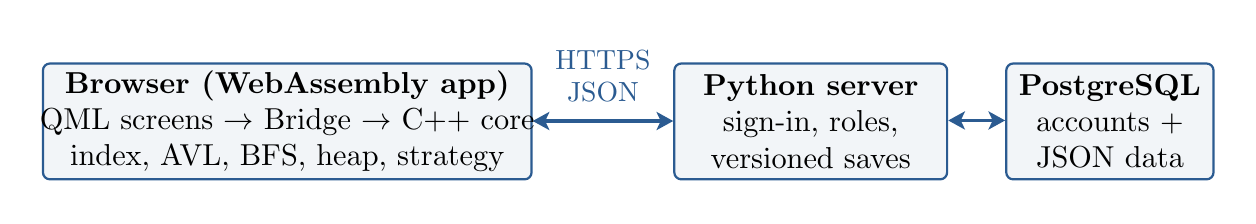
\begin{tikzpicture}[x=1bp,y=-1bp,
    dbox/.style={draw=GEUBlue,line width=0.8bp,fill=GEUBlue!6,rounded corners=2.5bp},
    dtxt/.style={inner sep=0pt,align=center,font=\fontsize{11bp}{13bp}\selectfont},
    darr/.style={GEUBlue,line width=1.1bp,{Stealth[length=6bp,width=6.5bp,inset=1.5bp]}-{Stealth[length=6bp,width=6.5bp,inset=1.5bp]}}]
  \useasboundingbox (0,0) rectangle (432,60.7);
  \draw[dbox] (5.5,12.9)   rectangle (181.4,54.6);
  \draw[dbox] (232.8,12.9) rectangle (331.0,54.6);
  \draw[dbox] (352.3,12.9) rectangle (426.9,54.6);
  \node[dtxt] at (93.45,33.75)
    {\textbf{Browser (WebAssembly app)}\\QML screens $\rightarrow$ Bridge $\rightarrow$ C++ core\\index, AVL, BFS, heap, strategy};
  \node[dtxt] at (281.9,33.75) {\textbf{Python server}\\sign-in, roles,\\versioned saves};
  \node[dtxt] at (389.6,33.75) {\textbf{PostgreSQL}\\accounts +\\JSON data};
  \draw[darr] (181.8,33.6) -- (232.4,33.6);
  \draw[darr] (331.4,33.4) -- (351.9,33.4);
  \node[inner sep=0pt,anchor=base,text=GEUBlue,font=\fontsize{9.5bp}{11.3bp}\selectfont,align=center]
    at (207.1,26.4) {HTTPS\\JSON};  % anchored on the last line (JSON)
\end{tikzpicture}\hss}
\end{answerbox}

\newpage
% ====================================================================
% PAGE 3 -- TASKS COMPLETED, CHALLENGES, TASKS PENDING
% ====================================================================
\TFpagetop
\TFsection{26.8bp}{Tasks Completed (7 pts)}
  {(Describe the main tasks that have been assigned and already completed. Max 250 words).}
\TFblock{6.1bp}{\TFtablefont
  \begin{tabular}[t]{|T{326.25bp}|T{138.55bp}|}
  \hline
  \rowcolor{TableHeadGrey}\textbf{Task Completed} & \textbf{Team Member}\\ \hline
  Data structures: \codes{SkillIndex} (hash map), \codes{SkillBST} (AVL tree with prefix search for
  autocomplete), \codes{SkillGraph} (BFS for related skills), top-\textit{k} ranking with a priority
  queue, greedy team suggestion. & Mehul (DSA Lead)\\ \hline
  Class design: \codes{Student}, \codes{ProjectRequirement}, \codes{Team}, \codes{InterestRequest};
  abstract \codes{MatchingStrategy} with weighted and coverage-only versions; \codes{Repository<T>}
  template; exception hierarchy; input validation. & Siddhant Singh (C++/OOP Lead)\\ \hline
  Qt Quick interface: entry screen with 3D logo, three workspaces, Match insights, 25 reusable
  components; 7 Qt Test programs; Windows test build with a testing checklist; documentation.
  & Anubhav Bisht (UI/Testing/Docs Lead)\\ \hline
  Integration: controller and permission model, interest workflow, JSON storage, session and log,
  CMake build. Web version: WebAssembly build, sign-in server, PostgreSQL storage, GitHub Actions
  build and Render deployment. & Mukul Fartiyal (Integration Lead)\\ \hline
  Sample data generator with a fixed seed: 560 participants, 8 projects, 549 skills, 86 interest
  requests. & Mukul Fartiyal, Mehul\\ \hline
  \end{tabular}}

\TFsection{24.2bp}{Challenges/Roadblocks (7 pts)}
  {(Describe the challenges that you have faced or are facing so far and how you plan to solve them. Max 300 words).}
\TFgap{6.1bp}
\begin{answerbox}
\begin{tfbullets}
\item \textbf{Availability factor:} we had no reliable timetable data, and scheduling made the screens
      confusing. We replaced it with engagement at the same weight and updated the expected scores in
      our tests.
\item \textbf{Keeping three structures in sync:} every profile change has to update the hash index, the
      AVL tree and the graph. We added rebuild functions and tests that check the rebuilt state matches
      the step-by-step state.
\item \textbf{Old sample data:} one build folder kept loading old data. We added a SHA-256 stamp and a
      backup before replacing files.
\item \textbf{First web version lost data:} our first Render site was a separate web app that saved to a
      local file. Render's free plan wipes local files on every restart, so accounts kept disappearing.
      We replaced it with the real Qt app and moved the data to PostgreSQL.
\item \textbf{Cloud build error (exit code 126):} a Qt helper script could not run on GitHub's machine.
      We changed the build to call CMake with Qt's toolchain file directly.
\item \textbf{App stopped on start in the browser:} Qt's ready-made WebAssembly kit turns off exception
      catching, but our core uses exceptions for validation. We enabled exception catching
      (\code{-fexceptions}) for our own code only, and the app now starts normally.
\item \textbf{Free hosting limits:} the site sleeps after 15 minutes without visitors, and the free
      database expires after 30 days. We will open the site before demos and move or upgrade the
      database before it expires.
\end{tfbullets}
\end{answerbox}

\TFsection{24.3bp}{Tasks Pending (7 pts)}
  {(Describe the main tasks that you still need to complete. Max 250 words).}
\TFblock{6.1bp}{\TFtablefont
  \begin{tabular}[t]{|T{326.25bp}|T{138.55bp}|}
  \hline
  \rowcolor{TableHeadGrey}\textbf{Task Pending} & \textbf{Team Member (to complete the task)}\\ \hline
  Run the full \codes{ctest} suite on the desktop build and record the results. & Anubhav Bisht\\ \hline
  Test the live site end to end with the testing checklist (sign up, edit profile, apply, build a team,
  reload) and fix any issues. & All members\\ \hline
  Compare the weighted strategy with the coverage-only baseline on the 560-profile dataset. & Mehul\\ \hline
  Move or upgrade the free database before it expires (about 9 November 2026). & Mukul Fartiyal\\ \hline
  Update the repository README (Phase II still says ``Upcoming''). & Anubhav Bisht\\ \hline
  Final demonstration, viva preparation and Phase III report. & All members\\ \hline
  \end{tabular}}

\newpage
% ====================================================================
% PAGE 4 -- OUTCOMES AND PROGRESS OVERVIEW
% ====================================================================
\TFpagetop
\TFsection{26.8bp}{Project Outcome/Deliverables (2 pts)}
  {(Describe what are the key outcomes / deliverables of the project. Max 200 words).}
\TFgap{6.1bp}
\begin{answerbox}
\begin{tfbullets}
\item A C++/Qt desktop application with Participant, Host and Developer workspaces.
\item A matching engine that finds candidates, scores them on five factors, ranks them, suggests a team
      and shows covered and missing skills.
\item Team validation for duplicate members, team size and missing skills.
\item Local JSON storage with sample data, backups and session restore.
\item A live website that runs the same app in the browser, with sign-in, roles and a shared PostgreSQL
      database.
\item An automatic build on GitHub Actions and deployment on Render.
\item Automated tests, a Windows test build, documentation and the DSA/OOP mapping for TCS-302 and
      TCS-307.
\end{tfbullets}
\end{answerbox}

\TFsection{27.8bp}{Progress Overview (2 pts)}
  {(Summarize how much of the project is done, what's behind schedule, what's ahead of schedule. Max 200 words.)}
\TFgap{6.1bp}
\begin{answerbox}
\begin{tfbullets}
\item \textbf{Done:} everything we planned for Phase II in our Phase I report: profiles, projects,
      candidate search, weighted matching and ranking, team building, skill gap checks, the data
      structures, the OOP design, local storage and automated tests.
\item \textbf{Ahead of schedule:} the interest workflow between participants and hosts, the Developer
      workspace that shows the data structures live, the 560-profile dataset, and the live website with
      sign-in.
\item \textbf{Behind schedule:} the recorded results of the full Qt test run, end-to-end testing on the
      live site, and the README update.
\item \textbf{Changed from the plan:} availability was replaced by engagement in the score.
\end{tfbullets}
\end{answerbox}

\newpage
% ====================================================================
% PAGE 5 -- CODEBASE, TESTING, DELIVERABLES
% ====================================================================
\TFpagetop
\TFsection{26.8bp}{Codebase Information (2 pts)}
  {(Repository link, branch, and information about important commits.)}
\TFgap{6.1bp}
\begin{answerbox}
\begin{tfbullets}
\item \textbf{Repository:} \TFurl{https://github.com/anubhav8it/TeamForge} (public), branch \code{main},
      45 commits as of 10 October 2026.
\item \textbf{Phase II code:} the \code{Phase-2/} folder contains \code{src/core}, \code{src/app},
      \code{src/web}, \code{ui/}, \code{tests/}, \code{data/}, \code{assets/}, \code{web/} (server and
      sign-in pages), \code{CMakeLists.txt} and \code{Dockerfile}.
\item \textbf{Important commits:} ``Add files via upload'' (Phase II source); ``Create build-web.yml'' and
      ``Update build-web.yml'' (automatic WebAssembly build); ``Create Dockerfile'' (Render deployment);
      ``Update CMakeLists.txt'' (exception fix for the browser build); ``Build TeamForge for
      WebAssembly'' (built files, committed by GitHub Actions).
\item \textbf{Live site:} \TFurl{https://teamforge-geu.onrender.com}
\end{tfbullets}
\end{answerbox}

\TFsection{27.8bp}{Testing and Validation Status (2 pts)}
  {(Provide information about any tests conducted)}
\TFblock{6.1bp}{\TFtablefont
  \begin{tabular}[t]{|T{146.15bp}|T{71.25bp}|T{236.15bp}|}
  \hline
  \rowcolor{TableHeadGrey}\textbf{Test Type} & \textbf{Status (Pass/Fail)} & \textbf{Notes}\\ \hline
  C++ core compile check (g++, \codes{-Wall -Wextra -Wpedantic}) & Pass & 15 core files compiled with 0 warnings.\\ \hline
  Unit and integration tests (Qt Test, \codes{ctest}) & To be recorded
    & 7 programs: domain, scoring, DSA, engine, persistence, controller, UI. Expected scores are worked out by hand.\\ \hline
  WebAssembly build (GitHub Actions) & Pass & First run failed (exit code 126); fixed. Later runs pass.\\ \hline
  Server API tests & Pass & 52 checks: sign-up, login, roles, re-login keeps data, conflicts, restart.\\ \hline
  Page sync logic & Pass & 11 checks: unchanged files skipped, changes saved, conflicts shown.\\ \hline
  Live site (10 Oct 2026) & Pass & Health check OK, sign-in works, admin account created, app opens on the entry screen.\\ \hline
  End-to-end use on the live site & In progress & Profile edit, reload and re-login with the testing checklist.\\ \hline
  \end{tabular}}

\TFsection{27.8bp}{Deliverables Progress (2 pts)}
  {(Summarize the current status of all key project deliverables mentioned earlier. Indicate whether each deliverable is completed, in progress, or pending.)}
\TFgap{17.1bp}% two-line instruction above
\begin{answerbox}
\begin{tfbullets}
\item Desktop application with three workspaces -- \textbf{Completed}
\item Matching engine (search, scoring, ranking, team suggestion, gap check) -- \textbf{Completed}
\item Team validation -- \textbf{Completed}
\item Local storage with sample data and backups -- \textbf{Completed}
\item Live website with sign-in and shared database -- \textbf{Completed}
\item Automatic build and deployment -- \textbf{Completed}
\item Automated tests -- \textbf{Completed}; recorded results -- \textbf{In progress}
\item Documentation and README update -- \textbf{In progress}
\item Strategy comparison, final demo and viva -- \textbf{Pending} (Phase III)
\end{tfbullets}
\end{answerbox}

\end{document}
